% Created 2022-12-04 Sun 20:51
% Intended LaTeX compiler: pdflatex
\documentclass[11pt]{article}
\usepackage[utf8]{inputenc}
\usepackage[T1]{fontenc}
\usepackage{graphicx}
\usepackage{longtable}
\usepackage{wrapfig}
\usepackage{rotating}
\usepackage[normalem]{ulem}
\usepackage{amsmath}
\usepackage{amssymb}
\usepackage{capt-of}
\usepackage{hyperref}
\usepackage[margin=0.85in]{geometry}
\date{}
\title{AST Exam Solutions}
\hypersetup{
 pdfauthor={Silent},
 pdftitle={AST Exam Solutions},
 pdfkeywords={},
 pdfsubject={},
 pdfcreator={Emacs 28.2 (Org mode 9.6)}, 
 pdflang={English}}
\begin{document}

\maketitle
\section{2018 Q3}
\label{sec:org8e3045b}
\subsection{Part (a)}
\label{sec:org2b0977c}
\begin{verbatim}
product []     = 1
product (0:_)  = 0
product (x:xs) = x * product xs
product [10,13,0,42]

product (10:[13,0,42])     = 10 * product [13,0,42] -- third case
10 * product (13:[0,42])   = 10 * (13 * product [0,42]) -- third case
10 * (13 * product (0:[42])) = 10 * (13 * 0) -- second case
\end{verbatim}
\begin{center}
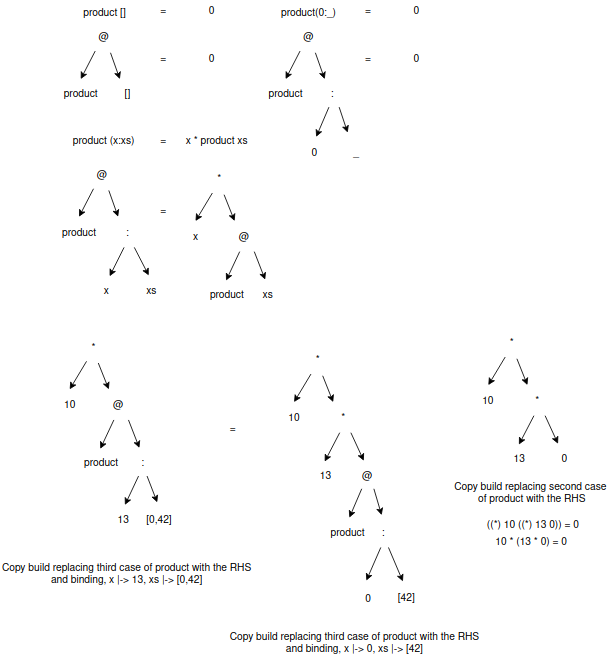
\includegraphics[width=115mm]{./product-xs.png}
\end{center}
\section{2018 Q3}
\label{sec:org674e1c4}
\subsection{Part (a)}
\label{sec:orgbbae674}
\begin{verbatim}
length [] = 0
length (x:xs) 1 + length xs
length [3,39]

length (3:[39])   = 1 + length [39] -- second case
1 + length ([39]) = 1 + (1 + length []) -- second case
1 + (1 length [])   = 1 + (1 + 0) -- first case
\end{verbatim}
\begin{center}
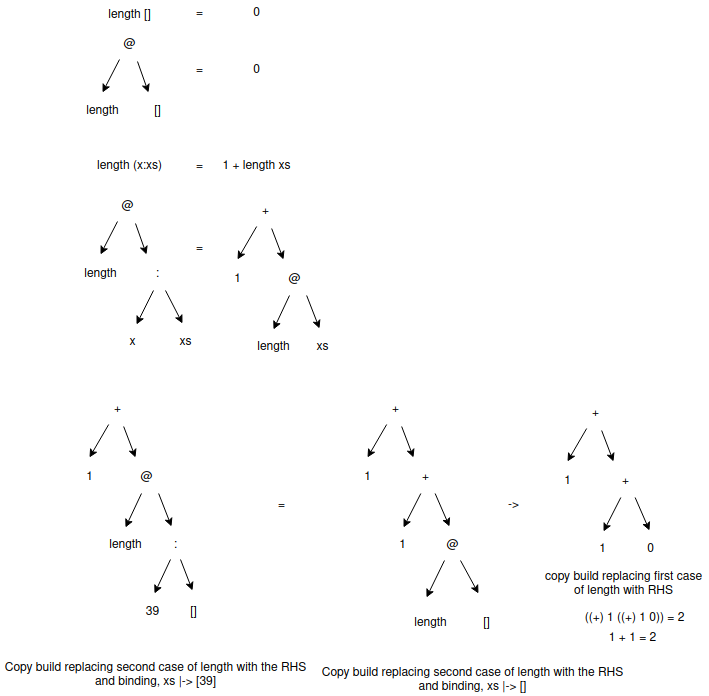
\includegraphics[width=160mm]{./length-xs.png}
\end{center}
\section{2016 Q3}
\label{sec:org3ba5018}
\subsection{Part (b)}
\label{sec:org48eeeaf}
\begin{verbatim}
prod []     = 1
prod (0:_)  = 0
prod (x:xs) = x * product xs
prod [3,14,0,999]

prod (3:[14,0,999])    = 3 * prod [14,0,999] -- third case
3 * product (13:[0,42])   = 3 * (14 * prod [0,42]) -- third case
3 * (13 * product (0:[42])) = 3 * (14 * 0) -- second case
\end{verbatim}
\begin{center}
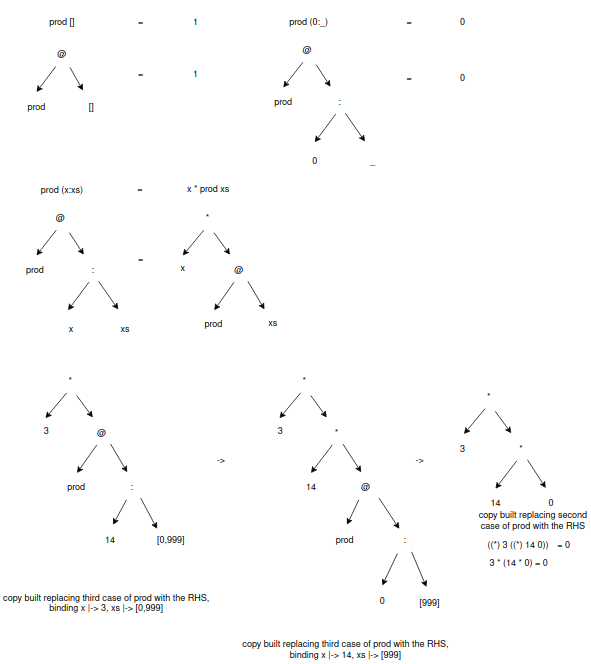
\includegraphics[width=155mm]{./prod-xs.png}
\end{center}
\section{2015 Q4}
\label{sec:orgaa7df96}
\subsection{Part (a)}
\label{sec:org783334c}
\begin{verbatim}
diffsq []     = 0
diffsq (x:xs) = x * x - diffsq xs
diffsq [2,3]

diffsq (2:[3])          = (2 * 2) - diffsq [3] -- second case
(2 * 2) - diffsq (3:[]) = (2 * 2) - ((3 * 3) - diffsq []) -- second case
(2 * 2) - ((3 * 3) - diffsq []) = (2 * 2) - ((3 * 3) - 0) -- first case
\end{verbatim}
\begin{center}
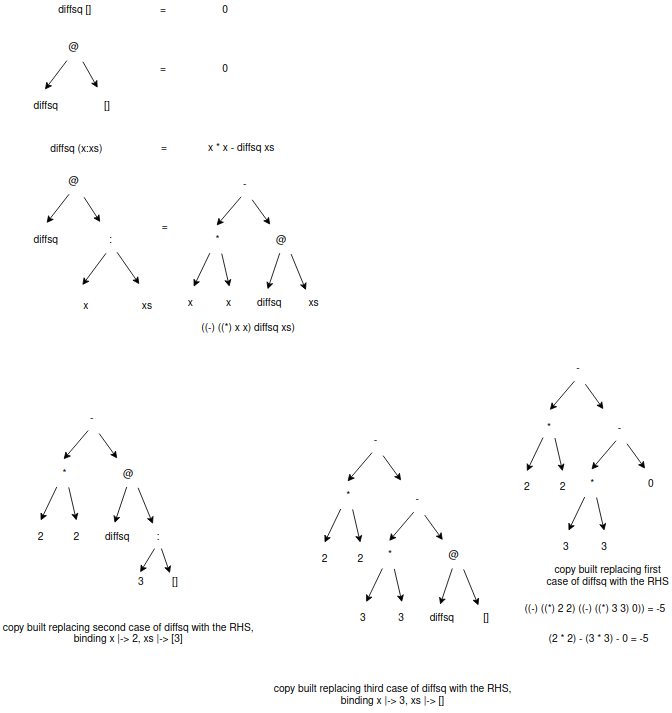
\includegraphics[width=160mm]{./diffsq-xs.png}
\end{center}
\section{2014 Q4}
\label{sec:orgd9fe989}
\subsection{Part (a)}
\label{sec:orge4a781f}
\begin{verbatim}
sum []     = 0
sum (x:xs) = x + sum xs
sum [3,39]

sum (3:[39])    = 3 + sum [39] -- second case
3 + sum (39:[]) = 3 + (39 + sum []) -- second case
3 + (39 + sum []) = 3 + (39 + 0) -- first case
\end{verbatim}
\begin{center}
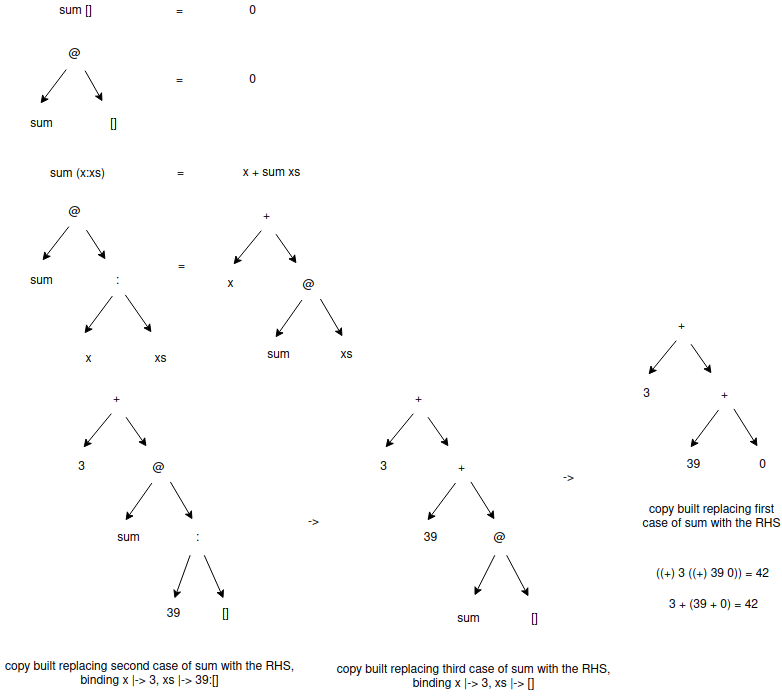
\includegraphics[width=160mm]{./sum-xs.png}
\end{center}
\newpage
\section{2013 Q4}
\label{sec:org4a3a311}
\subsection{Part (a)}
\label{sec:org11ea6e6}
\begin{verbatim}
sumsq []     = 0
sumsq (x:xs) = x * x - diffsq xs
sumsq [2,3]

sumsq (2:[3])           = (2 * 2) + diffsq [3] -- second case
(2 * 2) + sumsq (3:[]) = (2 * 2) + ((3 * 3) + sumsq []) -- second case
(2 * 2) + ((3 * 3) + sumsq []) = (2 * 2) + ((3 * 3) + 0) -- first case
\end{verbatim}
\begin{center}
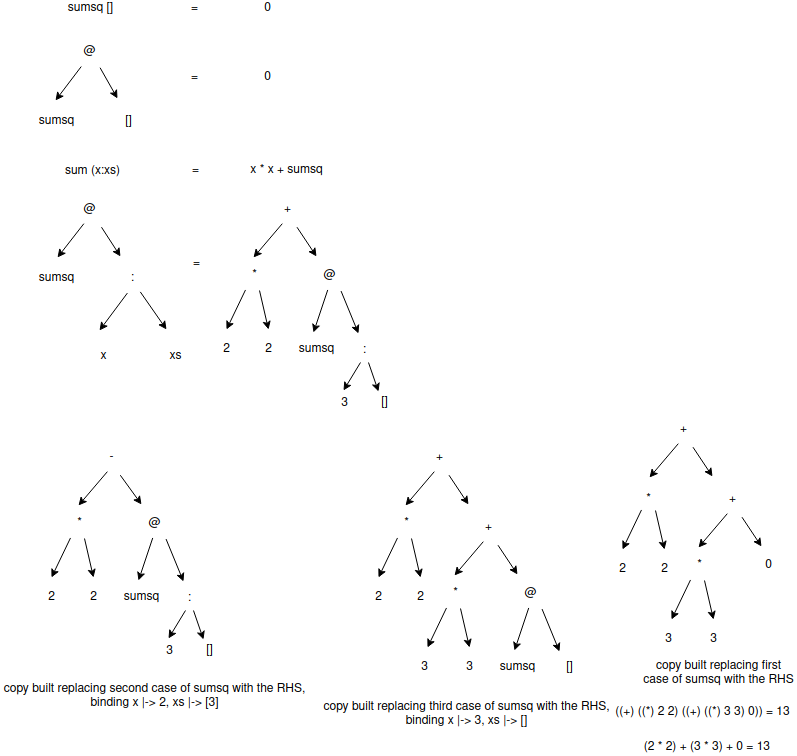
\includegraphics[width=160mm]{./sumsq-xs.png}
\end{center}
\end{document}